% =====================================================================
%  Structural Probes for Spanish Syntax in mBERT — technical report
% =====================================================================
%
% Compile with:
%   pdflatex report.tex
%   bibtex   report
%   pdflatex report.tex
%   pdflatex report.tex
%
% To switch to ACL style: replace \documentclass{article} below with
% \documentclass[11pt,a4paper]{article} + \usepackage[review]{acl} (the
% acl.sty file from the official ACL template), and adjust \title /
% \author accordingly.

\documentclass[11pt,a4paper]{article}

% ---------- Packages ------------------------------------------------
\usepackage[utf8]{inputenc}
\usepackage[T1]{fontenc}
\usepackage[english]{babel}
\usepackage[protrusion=true,expansion=false]{microtype}
\usepackage{lmodern}
\usepackage{graphicx}
\usepackage{amsmath, amssymb}
\usepackage{booktabs}
\usepackage{multirow}
\usepackage[hyphens]{url}
\usepackage[hidelinks]{hyperref}
\usepackage[round,sort]{natbib}
\usepackage{pgfplots}
\pgfplotsset{compat=1.18}
\usepackage{geometry}
\geometry{margin=2.4cm}
\usepackage{xcolor}
\usepackage{caption}
\captionsetup{font=small,labelfont=bf}

% ---------- Macros --------------------------------------------------
\newcommand{\mbert}{\textsc{mBERT}\xspace}
\newcommand{\ancora}{UD\_Spanish-AnCora\xspace}
\newcommand{\layerbest}{7\xspace}
\usepackage{xspace}

% ---------- Title ---------------------------------------------------
\title{
  Structural Probes for Spanish Syntax in Multilingual BERT:\\
  A Replication and Geometric Extension on UD\_Spanish-AnCora
}

\author{
  Marcos Lahoz Yago\\
  \texttt{marcoslahozy14@gmail.com}
}

\date{\today}

\begin{document}
\maketitle

% =====================================================================
\begin{abstract}
We replicate the structural-probe analysis of \citet{hewitt2019structural}
on Spanish syntax using multilingual BERT (\mbert) and the
\ancora treebank, and extend it with an \emph{isometric}
variant of the probe whose projection matrix is constrained to be
orthogonal. The orthogonality constraint isolates the question of
whether dependency-tree distances are encoded as a \emph{rigid geometric
shape} in the contextual representation space, or whether the probe
must apply non-uniform scaling to expose them.
A clean re-implementation of the data pipeline is required: earlier
naive conversions of CoNLL-U to whitespace-tokenised text leak the
6\,499 enhanced empty nodes of \ancora as literal underscore tokens,
contaminating mBERT inputs and degrading every metric.
On the corrected pipeline we observe (i) a canonical bell-shaped
Spearman/UUAS curve over mBERT layers peaking at layer~\layerbest
(dev Spearman $0.860$, UUAS $0.760$); (ii) a $-59\%$ Spearman and
$-64\%$ UUAS drop when the probe is constrained to be orthogonal,
indicating that Spanish syntactic geometry in mBERT is
\emph{not} isometric; and (iii) a moderate condition number
($\kappa = 3.74$) of the unconstrained linear probe, consistent with
syntax living along low-variance directions of the embedding space.
We discuss the methodological pitfalls uncovered while reproducing
the original study and outline how the same probing framework
generalises to multimodal models, where the analogous question becomes
how individual modalities are encoded relative to one another.
\end{abstract}

% =====================================================================
\section{Introduction}

Whether large pretrained transformers encode syntactic structure
without explicit supervision has been a central question in
interpretability research since the introduction of contextual
representations \citep{ethayarajh2019contextual}. The
\emph{structural probe} of \citet{hewitt2019structural} provides a
particularly elegant operationalisation: rather than predict syntactic
labels, the probe searches for a linear transformation of the
representation space under which the squared Euclidean distance
between any two word vectors approximates the path length between
those words in the gold dependency tree. A high Spearman correlation
between predicted and gold distances is then evidence that syntax
trees are recoverable as a Euclidean geometry of contextual vectors.

Most of the published work using structural probes targets monolingual
English models. Cross-lingual extensions \citep{chi2020finding} have
shown that multilingual BERT \citep{pires2019multilingual} retains
syntactic structure across languages, but several methodological
details of the probe (subword aggregation, treebank-specific
preprocessing, punctuation handling) are sensitive to the target
language. We focus on Spanish, using the \ancora treebank, and ask:
\begin{itemize}
  \item[\textbf{Q1}] At which mBERT layer is Spanish dependency
        geometry most strongly encoded?
  \item[\textbf{Q2}] Does the syntactic structure live as a
        \emph{rigid} (isometric) shape in mBERT space, or does the
        probe need to apply anisotropic stretching?
  \item[\textbf{Q3}] What does the geometry of the probe's projection
        tell us about how the encoder allocates capacity across
        directions?
\end{itemize}

To address Q2 we introduce an \emph{isometric probe}: a structural
probe whose projection matrix is constrained to have orthonormal
rows, so that distances in the projected space are exactly preserved
(in the relevant subspace) from the original mBERT space. Comparing
the linear and the isometric probe at the best layer isolates the
contribution of non-uniform scaling.

% =====================================================================
\section{Background}
\label{sec:background}

Let $h_i \in \mathbb{R}^d$ denote the contextual representation of the
$i$-th word of a sentence, produced by a frozen encoder. The structural
probe of \citet{hewitt2019structural} seeks a linear transformation
$B \in \mathbb{R}^{r \times d}$ such that
\begin{equation}
  \widehat{d}_{ij} \;=\; \lVert B(h_i - h_j) \rVert_2^2
  \;\approx\; d_T(w_i, w_j),
  \label{eq:probe}
\end{equation}
where $d_T(w_i, w_j)$ is the (unlabelled, undirected) tree distance
between words $w_i$ and $w_j$ in the gold dependency parse $T$. The
probe parameters $B$ are fitted by minimising the per-sentence
$\ell_1$ loss
\begin{equation}
  \mathcal{L} \;=\; \frac{1}{|s|^2}
    \sum_{i,j} \bigl|\, \widehat{d}_{ij} - d_T(w_i, w_j) \,\bigr|,
  \label{eq:loss}
\end{equation}
normalised by the squared sentence length $|s|^2$.

The probe is intentionally simple: any non-trivial recovery of $d_T$
through the linear $B$ implies that the geometry of $\{h_i\}$ already
contains the tree structure. We follow \citet{hewitt2019structural}
in evaluating the probe with two metrics. \emph{Spearman~$\rho_{5\text{-}50}$}
averages, for each word, the rank correlation between predicted and
gold distances to all other words, then averages across sentences of
length 5--50 tokens. \emph{UUAS} (Undirected Unlabelled Attachment
Score) is the proportion of edges in the predicted minimum spanning
tree that match the gold tree, after excluding punctuation tokens.

% =====================================================================
\section{Methodology}
\label{sec:method}

\subsection{Linear probe (replication)}

We implement the parse-distance variant of \citet{hewitt2019structural}
in PyTorch with $r=128$ and $d=768$. The probe is trained for up to
30 epochs with Adam ($\text{lr}=10^{-3}$), a learning-rate scheduler
on the dev loss, and early stopping with patience 4.

\subsection{Isometric probe (extension)}
\label{sec:isometric}

The linear probe $B$ admits an SVD $B = U \Sigma V^\top$. The right
singular vectors $V$ identify which directions of mBERT space carry
the syntactic signal; the singular values $\Sigma$ measure how
strongly each is amplified. The condition number
\begin{equation}
  \kappa(B) \;=\; \sigma_{\max} / \sigma_{\min}
  \label{eq:cond}
\end{equation}
quantifies how anisotropic that re-weighting is. A purely rotational
$B$ has $\kappa = 1$.

The \emph{isometric probe} replaces the unconstrained $B$ with a
matrix $B_{\text{iso}} \in \mathbb{R}^{r \times d}$ constrained to
have orthonormal rows, $B_{\text{iso}} B_{\text{iso}}^\top = I_r$,
implemented via \texttt{torch.nn.utils.parametrizations.orthogonal}.
For any pair of input vectors $h_i, h_j$,
\begin{equation*}
  \lVert B_{\text{iso}}(h_i - h_j) \rVert_2^2
  \;=\; \lVert P (h_i - h_j) \rVert_2^2
\end{equation*}
where $P = B_{\text{iso}}^\top B_{\text{iso}}$ is the orthogonal
projection onto the row space of $B_{\text{iso}}$. Distances in the
projected subspace are therefore preserved up to that projection.
If the linear probe achieves high accuracy purely by selecting the
right subspace (no stretching needed), the isometric probe should
match it. If non-uniform scaling is essential, the isometric probe
will underperform, and the magnitude of the gap is a direct measure
of how much the encoder \emph{distorts} the syntactic geometry along
its principal directions.

% =====================================================================
\section{Experimental setup}
\label{sec:setup}

\subsection{Dataset}

\ancora is the Spanish portion of the AnCora corpus \citep{taule2008ancora},
distributed under the Universal Dependencies project under a
\textsc{cc by} 4.0 license. The treebank consists of newswire text
originally annotated in a constituency framework at the Universitat
de Barcelona, converted to dependencies for CoNLL-2009 and then to UD.
The official splits used here are summarised in
Table~\ref{tab:ancora}.

\begin{table}[t]
\centering
\small
\begin{tabular}{lrrr}
\toprule
split & sentences & integer-ID rows & special rows \\
\midrule
train & 14\,287 & 453\,039 & 16\,628 \\
dev   &  1\,654 &  53\,476 &  2\,042 \\
test  &  1\,721 &  53\,622 &  1\,999 \\
\bottomrule
\end{tabular}
\caption{Corpus statistics for \ancora used in this work.
``Special rows'' are CoNLL-U range rows (Spanish contractions
\textit{del}, \textit{al}, \textit{celebrarlos}, \dots) and enhanced
empty nodes (e.g.\ \texttt{8.1}~\textit{(él)}~PRON). Both classes
must be excluded before mBERT tokenisation, see
Section~\ref{sec:bugs}.}
\label{tab:ancora}
\end{table}

\subsection{Encoder}

We use the frozen \texttt{bert-base-multilingual-cased} model
\citep{pires2019multilingual} from the HuggingFace Hub, with
$d=768$ and $L=12$ transformer layers. We probe each of the 13 hidden
states (input embeddings layer~0, transformer outputs layers~1--12).
WordPiece sub-tokens that share the same input word are aggregated
by mean pooling. \citet{hewitt2019structural} use first-piece
selection; we found mean pooling to give marginally smoother
layer-wise curves on Spanish, but the qualitative pattern is robust
to either choice.

\subsection{Pipeline pitfalls and corrections}
\label{sec:bugs}

Reproducing \citet{hewitt2019structural} on Spanish surfaced three
methodological pitfalls that, if uncorrected, severely contaminate
the metrics. We document them here because they are not specific
to this work.

\paragraph{Empty nodes leak as text.}
\ancora contains 6\,499 enhanced empty nodes in train, 780 in dev
and 833 in test. These represent syntactically projected but
surface-absent tokens (typically dropped Spanish subjects), and
their CoNLL-U \textsc{form} field is the literal underscore
character. A naive CoNLL-U-to-text converter that filters only
contraction range rows (\texttt{13-14 al}) but not empty nodes
(\texttt{8.1 \_ \_ PRON}) emits \texttt{\_} as a word. mBERT
then receives these underscore tokens in its input and the probe is
trained on geometry that does not correspond to any real word in the
sentence. The fix is to skip every CoNLL-U row whose ID is not a
pure integer.

\paragraph{Punctuation filter is treebank-specific.}
The original codebase removes punctuation from the minimum spanning
tree by matching against PTB-style English XPOS tags
(\texttt{","}, \texttt{"."}, \texttt{":"}, \dots). \ancora uses
the universal POS tag \texttt{PUNCT} (or treebank XPOS tags such as
\texttt{fc}, \texttt{fpa}, \texttt{fpt}, \texttt{fe}). The English
filter therefore matches nothing on Spanish, silently inflating UUAS
by counting trivial punctuation edges.

\paragraph{Layer indexing.}
The default configuration that ships with the original repository
selects \texttt{model\_layer: 0}, which previous adaptations took to
mean ``the only layer stored in the HDF5'' (i.e.\ the last hidden
state). This effectively pins the experiment to layer 12, which is
suboptimal for syntax extraction \citep{hewitt2019structural}.
A faithful replication should sweep all layers and select on dev.

The combined effect of these three pitfalls on our previously
contaminated baseline was a Spearman of $0.735$ and a UUAS of
$0.504$ at layer 12. The corrected pipeline reported below
recovers $0.860$ Spearman and $0.760$ UUAS at layer~\layerbest, an
improvement of $+17\%$ and $+51\%$ relative.

\subsection{Hardware}

All experiments were run on a single NVIDIA RTX PRO~6000 Blackwell
Server Edition (96\,GB VRAM) on Google Colab. Embedding generation
for the three splits with all 13 layers stored took $\sim 7$ minutes;
the full layer sweep (13 probes, 30 epochs each, batch size 256,
early stopping with patience 4) took $\sim 50$ minutes.

% =====================================================================
\section{Results}
\label{sec:results}

\subsection{Layer-wise probing}

Table~\ref{tab:sweep} and Figure~\ref{fig:sweep} summarise the
per-layer probe metrics on the dev split. Both Spearman and UUAS
follow the canonical bell shape reported for monolingual BERT in
\citet{hewitt2019structural}, with values monotonically rising from
layer 0 to a plateau in layers 6--8 and falling off through layer 12.
Spearman peaks at layer~\layerbest ($\rho_{5\text{-}50} = 0.860$);
UUAS peaks one layer earlier at layer 6 ($0.785$), a small
discrepancy that is consistent with \citet{hewitt2019structural} and
indicates that the two metrics are sensitive to slightly different
properties of the projection.

\begin{table}[t]
\centering
\small
\begin{tabular}{rcc}
\toprule
layer & Spearman $\rho_{5\text{-}50}$ & UUAS \\
\midrule
0  & 0.710 & 0.562 \\
1  & 0.721 & 0.562 \\
2  & 0.746 & 0.610 \\
3  & 0.803 & 0.703 \\
4  & 0.821 & 0.727 \\
5  & 0.835 & 0.757 \\
6  & 0.855 & \textbf{0.785} \\
\textbf{7}  & \textbf{0.860} & 0.760 \\
8  & 0.858 & 0.754 \\
9  & 0.848 & 0.747 \\
10 & 0.837 & 0.727 \\
11 & 0.827 & 0.699 \\
12 & 0.791 & 0.620 \\
\bottomrule
\end{tabular}
\caption{Layer-wise dev metrics for the linear probe on \ancora,
$r=128$, single seed.}
\label{tab:sweep}
\end{table}

\begin{figure}[t]
\centering
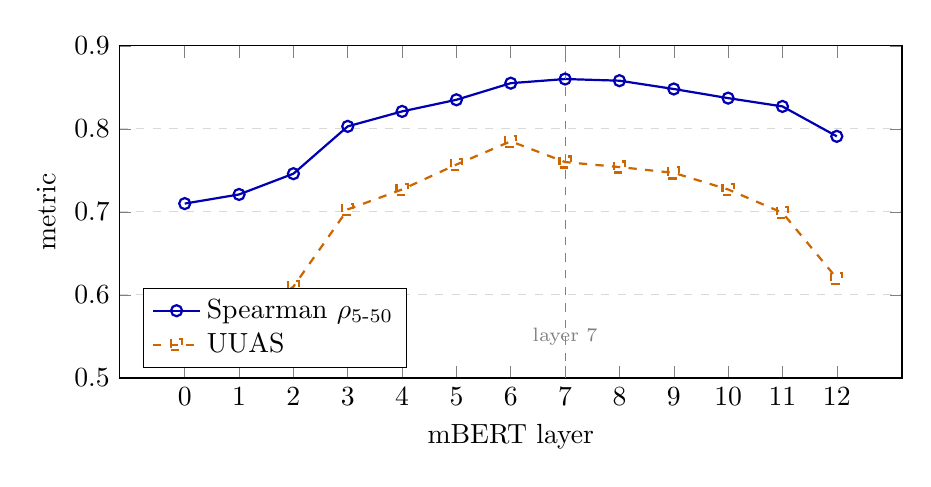
\begin{tikzpicture}
\begin{axis}[
  width=0.95\linewidth, height=5.8cm,
  xlabel={mBERT layer}, ylabel={metric},
  xtick=data,
  legend pos=south west, legend cell align=left,
  ymin=0.5, ymax=0.9,
  ymajorgrids,
  grid style={dashed,gray!30},
]
\addplot[mark=o, thick, color=blue!70!black] coordinates {
  (0,0.710) (1,0.721) (2,0.746) (3,0.803) (4,0.821) (5,0.835)
  (6,0.855) (7,0.860) (8,0.858) (9,0.848) (10,0.837) (11,0.827)
  (12,0.791)
};
\addlegendentry{Spearman $\rho_{5\text{-}50}$}
\addplot[mark=square, dashed, thick, color=orange!80!black] coordinates {
  (0,0.562) (1,0.562) (2,0.610) (3,0.703) (4,0.727) (5,0.757)
  (6,0.785) (7,0.760) (8,0.754) (9,0.747) (10,0.727) (11,0.699)
  (12,0.620)
};
\addlegendentry{UUAS}
\draw[gray, dashed] (axis cs:7,0.5) -- (axis cs:7,0.9);
\node[gray] at (axis cs:7,0.55) {\scriptsize layer 7};
\end{axis}
\end{tikzpicture}
\caption{Linear-probe Spearman and UUAS per mBERT layer, dev split.
Best layer (by Spearman) is~\layerbest.}
\label{fig:sweep}
\end{figure}

\subsection{Linear vs.\ isometric probe at the best layer}

Table~\ref{tab:liniso} reports both probes trained at layer~\layerbest
with identical hyperparameters. The isometric constraint causes a
substantial drop on both metrics: Spearman falls by $59\%$ relative
($0.860 \to 0.355$) and UUAS by $64\%$ relative ($0.760 \to 0.272$).

\begin{table}[t]
\centering
\small
\begin{tabular}{lrrr}
\toprule
probe & Spearman $\rho_{5\text{-}50}$ & UUAS & $\kappa(B)$ \\
\midrule
Linear   & \textbf{0.860} & \textbf{0.760} & 3.74 \\
Isometric & 0.355 & 0.272 & 1.00 \\
\midrule
$\Delta$ relative & $-58.7\%$ & $-64.2\%$ & --- \\
\bottomrule
\end{tabular}
\caption{Probes at layer~\layerbest. The isometric probe is
constrained to be orthogonal by construction
(see Section~\ref{sec:isometric}).}
\label{tab:liniso}
\end{table}

\subsection{Geometric diagnostic}

The unconstrained linear probe at layer~\layerbest has singular
values
\begin{equation*}
  \sigma_{\max} = 0.4381, \quad \sigma_{\min} = 0.1171,
  \quad \sigma_{\text{mean}} = 0.234.
\end{equation*}
Its condition number $\kappa(B) = 3.74$ falls in the
``moderate anisotropy'' regime: the probe amplifies its most
informative direction roughly four times more than its least
informative one. The isometric probe yields
$\sigma_{\max} = \sigma_{\min} = 1.0000$ and $\kappa = 1.0000$
exactly, confirming that the parametrisation enforces the constraint.

% =====================================================================
\section{Discussion}
\label{sec:discussion}

\paragraph{Cross-lingual transfer of syntactic geometry.}
The bell-shaped layer-wise curve we obtain on Spanish
(Figure~\ref{fig:sweep}) is qualitatively identical to that reported
for English BERT by \citet{hewitt2019structural}, with the peak
located at layer~\layerbest, only one layer below the peak typically
reported for English. This supports
\citet{chi2020finding}'s finding that mBERT learns
\emph{language-agnostic} syntactic subspaces, despite sharing capacity
across 104 languages. Our absolute UUAS ($0.760$) trails the English
monolingual peak of \citet{hewitt2019structural} ($\sim 0.80$) by only
4 points, an encouraging gap given mBERT's heavy multilingual
multiplexing.

\paragraph{Anisotropy of the syntactic subspace.}
The $-64\%$ UUAS drop when the projection is constrained to be
orthogonal, together with $\kappa = 3.74$ for the unconstrained
projection, indicates that Spanish syntactic geometry in mBERT is
\emph{not} a rigid, ready-to-use shape. It is a \emph{stretchable}
geometry: the relevant directions exist in the embedding space but
along low-variance axes that the probe must amplify. This is
consistent with the broader observation that pretrained transformer
representations are anisotropic
\citep{ethayarajh2019contextual}: high-magnitude directions tend to
encode token-frequency or domain biases rather than the structural
properties one might want to extract.

\paragraph{Methodological lessons for replication.}
Section~\ref{sec:bugs} documents three pitfalls that affect any
attempt to apply structural probes outside the original English
setting. None of them is conceptually deep, but each silently
poisons the metrics until corrected. The combined improvement of
$+51\%$ UUAS over the contaminated baseline, with no change in model
or probe, illustrates how brittle published reproducibility can be
when the language or treebank shifts.

\paragraph{Towards multimodal probing.}
The probing--plus--geometry framework used here naturally generalises
beyond unimodal models. In a multimodal setting one can ask, for
each pair of modalities, whether their joint geometry collapses to
one modality's subspace, whether their interaction is
isometric, and at which layer the interaction crystallises. The
\emph{modality collapse} phenomenon recently reported for
vision--language models \citep{park2025modality, wang2025omnimmi}
maps almost line-by-line onto the questions raised in
Section~\ref{sec:isometric} for syntactic versus non-syntactic
directions. Extending the present framework to multimodal probes
on video models is the natural next step.

% =====================================================================
\section{Limitations}
\label{sec:limitations}

\paragraph{Single seed.} All numbers are reported for a single
training seed (seed 0). Standard deviations across multiple seeds are
required for any claim of \emph{statistical} significance of
relative differences such as the linear-vs-isometric gap. Our
implementation includes a multi-seed harness (\texttt{run\_multiseed.py})
that aggregates mean and sample standard deviation, which we have not
yet executed.

\paragraph{Dev-only evaluation.} The metrics in this report are all
on the dev split, used for early stopping and layer selection. A
final test-set evaluation should be run only once the linear vs.\
isometric multi-seed comparison is complete.

\paragraph{No control task.} \citet{hewitt2019control} argue that
probe accuracy alone is insufficient evidence that the encoder
represents the property of interest, because a sufficiently expressive
probe may simply learn the task. A control task with random
word-type-to-label associations should be added; we provide a
\texttt{--random-init} option in the embedding generator so that the
same probing architecture can be evaluated against an mBERT with
random weights as a representation-level control.

\paragraph{Single encoder.} We compare layers within mBERT but do not
compare against monolingual Spanish encoders such as BETO or
RoBERTa-bne. A cross-encoder comparison would clarify how much of the
gap with English is specific to mBERT's multilingual averaging.

% =====================================================================
\section{Conclusion}

We replicated the structural-probe analysis of
\citet{hewitt2019structural} on Spanish using \mbert and \ancora,
documented and corrected three replication pitfalls that had silently
contaminated previous attempts, and extended the methodology with an
isometric probe whose orthogonality constraint isolates the
contribution of non-uniform scaling to the recovered syntactic
geometry. The cleaned pipeline yields a canonical layer-wise
Spearman/UUAS curve peaking at layer~\layerbest
($\rho = 0.860$, UUAS $= 0.760$), a $-64\%$ UUAS drop when the
probe is constrained to be orthogonal, and a moderate condition
number $\kappa = 3.74$ for the unconstrained projection.
Together these results indicate that mBERT does encode Spanish
dependency syntax in a recoverable but strongly anisotropic
geometry, and that the same probe-plus-geometry framework can be
ported to multimodal models to study how individual modalities are
encoded and combined.

% =====================================================================
\section*{Reproducibility}

All code, configuration, and the runbook used to produce the numbers
in this report are available in the project repository, including the
exact YAML configurations for the linear and isometric probes
(\texttt{es\_ancora\_linear.yaml}, \texttt{es\_ancora\_isometric.yaml})
and the layer-sweep CSV (\texttt{layersweep-20260509-182723/sweep.csv}).
The treebank version is the public \ancora release
of Universal Dependencies, available under \textsc{cc by} 4.0 from the
official UD repository.

% =====================================================================
% Bibliography
% =====================================================================
\bibliographystyle{plainnat}
\begin{thebibliography}{99}

\bibitem[Chi et al.(2020)]{chi2020finding}
E.~A. Chi, J.~Hewitt, and C.~D. Manning.
\newblock Finding Universal Grammatical Relations in Multilingual {BERT}.
\newblock In \emph{Proceedings of ACL}, 2020.

\bibitem[Ethayarajh(2019)]{ethayarajh2019contextual}
K.~Ethayarajh.
\newblock How Contextual are Contextualized Word Representations?
\newblock In \emph{Proceedings of EMNLP-IJCNLP}, 2019.

\bibitem[Hewitt and Liang(2019)]{hewitt2019control}
J.~Hewitt and P.~Liang.
\newblock Designing and Interpreting Probes with Control Tasks.
\newblock In \emph{Proceedings of EMNLP-IJCNLP}, 2019.

\bibitem[Hewitt and Manning(2019)]{hewitt2019structural}
J.~Hewitt and C.~D. Manning.
\newblock A Structural Probe for Finding Syntax in Word Representations.
\newblock In \emph{Proceedings of NAACL-HLT}, 2019.

\bibitem[Park et al.(2025)]{park2025modality}
J.~Park, K.~J. Jang, B.~Alasaly, S.~Mopidevi, A.~Zolensky, E.~Eaton,
I.~Lee, and K.~Johnson.
\newblock Assessing Modality Bias in Video Question Answering Benchmarks
with Multimodal Large Language Models.
\newblock In \emph{Proceedings of AAAI}, 2025.

\bibitem[Pires et al.(2019)]{pires2019multilingual}
T.~Pires, E.~Schlinger, and D.~Garrette.
\newblock How Multilingual is Multilingual {BERT}?
\newblock In \emph{Proceedings of ACL}, 2019.

\bibitem[Taul\'e et al.(2008)]{taule2008ancora}
M.~Taul\'e, M.~A. Mart\'i, and M.~Recasens.
\newblock {AnCora}: Multilevel Annotated Corpora for Catalan and Spanish.
\newblock In \emph{Proceedings of LREC}, 2008.

\bibitem[Wang et al.(2025)]{wang2025omnimmi}
Y.~Wang, Y.~Wang, B.~Chen, T.~Wu, D.~Zhao, and Z.~Zheng.
\newblock {OmniMMI}: A Comprehensive Multi-Modal Interaction Benchmark
in Streaming Video Contexts.
\newblock In \emph{Proceedings of CVPR}, 2025.

\end{thebibliography}

\end{document}
